\documentclass[11pt,openany,twoside]{report}
%%%%%%%%%%%%%%%%%%%%%%%%%%%%%%%%%%%%%%%%%%%%%%%%%%%%%%%%%%%%%%%%%%%%
%%		packages	%%%%%%%%%%%%%%%%%%%%%%%%%%%%%%%%%%%%%%%%%%%%%%%%
%%%%%%%%%%%%%%%%%%%%%%%%%%%%%%%%%%%%%%%%%%%%%%%%%%%%%%%%%%%%%%%%%%%%
\usepackage[utf8]{inputenc}
\usepackage[hmargin=4cm,vmargin=3.5cm,bmargin=3.5cm]{geometry}
\usepackage[portuguese, english]{babel}
\usepackage{graphicx}
\usepackage{hyperref}
\usepackage{indentfirst}
\usepackage{acronym}
%%%%%%%%%%%%%%%%%%%%%%%%%%%%%%%%%%%%%%%%%%%%%%%%%%%%%%%%%%%%%%%%%%%%
%%		package listings - para por o código no relatório %%%%%%%%%
%%%%%%%%%%%%%%%%%%%%%%%%%%%%%%%%%%%%%%%%%%%%%%%%%%%%%%%%%%%%%%%%%%%%
\usepackage{listings}
\usepackage{color}
\definecolor{codegreen}{rgb}{0,0.6,0}
\definecolor{codegray}{rgb}{0.5,0.5,0.5}
\definecolor{codepurple}{rgb}{0.58,0,0.82}
\definecolor{backcolour}{rgb}{0.9,0.9,0.9}
\definecolor{lightgray}{rgb}{.9,.9,.9}
\definecolor{darkgray}{rgb}{.4,.4,.4}
\definecolor{purple}{rgb}{0.65, 0.12, 0.82}
\lstdefinestyle{mystyle}{
    backgroundcolor=\color{lightgray},
    commentstyle=\color{purple}\ttfamily,
    keywordstyle=\color{blue}\bfseries,
    numberstyle=\footnotesize,
    stringstyle=\color{red}\ttfamily,
    basicstyle=\footnotesize,
    breakatwhitespace=false,         
    breaklines=true,                 
    captionpos=b,                    
    keepspaces=true,                 
    numbers=left,                    
    numbersep=5pt,                  
    showspaces=false,                
    showstringspaces=false,
    showtabs=false,                  
    tabsize=2
}
\lstset{style=mystyle}
\lstset{literate={ą}{{\k{a}}}1 {ç}{{\'c}}1 {ę}{{\k{e}}}1 {ł}{{\l{}}}1 {ń}{{\'n}}1 {ó}{{\'o}}1 {ś}{{\'s}}1 {ż}{{\.z}}1 {ź}{{\'z}}1 {Ą}{{\k{A}}}1 {Ć}{{\'C}}1 {Ę}{{\k{E}}}1 {Ł}{{\L{}}}1 {Ń}{{\'N}}1 {Ó}{{\'O}}1 {Ś}{{\'S}}1 {Ż}{{\.Z}}1 {Ź}{{\'Z}}1 {í}{{\'i}}1 {á}{{\'a}}1
{Á}{{\'A}}1 {é}{{\'e}}1 {É}{{\'E}}1 {Í}{{\'I}}1 {ú}{{\'u}}1 {Ú}{{\'U}}1 {ã}{{a}}1 {õ}{{o}}1 {à}{{a}}1}
%%%%%%%%%%%%%%%%%%%%%%%%%%%%%%%%%%%%%%%%%%%%%%%%%%%%%%%%%%%%%%%%%%%%
%%   	CABEÇALHO E CAPA			%%%%%%%%%%%%%%%%%%%%%%%%%%%%%%%%
%%%%%%%%%%%%%%%%%%%%%%%%%%%%%%%%%%%%%%%%%%%%%%%%%%%%%%%%%%%%%%%%%%%%

\title{\textbf{Projeto 2 - Relatório Final}}

\begin{document}

\begin{titlepage}
\begin{figure}
\title{\textbf{Projeto 2 - Relatório Final}}
\author{\\\vspace{0.3cm}
Abel Fernandes Neto
\\\vspace{0.3cm}
Daniel Azevedo Alves
\\\vspace{0.3cm}
Diogo Daniel Soares Ferreira
\\\vspace{0.3cm} 
Luís Davide Jesus Leira
\\\vspace{0.3cm}
\textbf{Universidade de Aveiro - Laboratórios de Informática - Grupo 3}}
\date{\today}
 
\includegraphics[scale=1.5]{ua_logo.png}
\end{figure}
\end{titlepage}

\selectlanguage{portuguese}
\maketitle
\tableofcontents
\listoffigures
%%%%%%%%%%%%%%%%%%%%%%%%%%%%%%%%%%%%%%%%%%%%%%%%%%%%%%%%%%%%%%%%%%%%
%%		Ínicio do Relatório		%%%%%%%%%%%%%%%%%%%%%%%%%%%%%%%%%%%%
%%%%%%%%%%%%%%%%%%%%%%%%%%%%%%%%%%%%%%%%%%%%%%%%%%%%%%%%%%%%%%%%%%%%

\part{Apresentação}

\chapter{Resumo}
\paragraph{ } Este relatório consiste na identificação dos objetivos propostos, na análise à estrutura da aplicação, na descrição da implementação efetuada e nas conclusões finais sobre a solução implementada. Encontram-se em anexo os testes realizados à aplicação. 

O objetivo deste projeto é desenvolver uma aplicação \textit{web} capaz de replicar o funcionamento de um órgão de \textit{Hammond} (\autoref{hammond}). Através de pautas em formato \ac{rtttl}, a aplicação deverá ser capaz de reproduzir o respetivo som, de acordo com um registo passado pelo utilizador e de efeitos adicionais opcionais. A aplicação é composta por cinco módulos principais: a interface \textit{Web}, a aplicação principal, o sintetizador, o interpretador de pautas e o processador de efeitos. O repositório utilizado para o desenvolvimento da aplicação está alojado no \textit{CodeUA} e o seu nome é "labi2015-proj2-g3".

\begin{figure}
 \center
 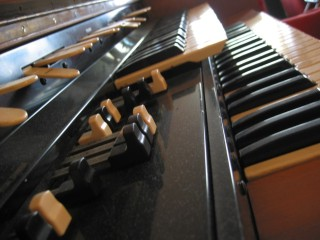
\includegraphics[scale=.6]{Hammond_l100.jpg}
 \caption{Órgão de \textit{Hammond}. Fonte: Wikipédia}
 \label{hammond}
\end{figure}

\part{Desenvolvimento}

\chapter{Estrutura}

\paragraph{ } Uma aplicação \textit{Web} baseia-se numa página web, normalmente apresentada num \textit{browser}, onde o utilizador poderá executar alguma tarefa para além de apenas ler o conteúdo da página. O utilizador poderá interagir com a página, a qual se encarrega de efetuar pedidos ao servidor, o qual tem como objetivo ser a base da aplicação, efetuando as respostas aos pedidos realizados e que transmite ao utilizador (caso seja necessário). As aplicações \textit{Web} devem visar pela sua simplicidade e pelo cumprimento de tarefas de forma direta e eficaz.

A interface \textit{Web} encontra-se disponível numa versão \textit{desktop} e numa versão \textit{mobile}. O código \textit{JavaScript} considera-se essencial em ambas as versões. A interface deverá permitir ao utilizador criar  músicas e versões das mesmas (podendo alterar os efeitos e os registos aplicados inicialmente aquando da criação da música), listar as músicas e versões existentes, aceder a informações básicas de todas as versões das músicas criadas, obter um gráfico das notas, poder ouvir cada versão através de um ficheiro áudio e atribuir votos positivos ou negativos a cada versão. A interface \textit{Web} deverá comunicar com o servidor através de mensagens no formato \ac{json}.

A aplicação principal tem como módulo principal o \textit{Cherrypy}. Deverá assegurar que responde corretamente aos pedidos realizados pelo utilizador da aplicação. Também deve criar um gráfico de notas quando pedido (através do módulo de \textit{python matplotlib}) e disponibilizar ficheiros áudio que o utilizador poderá reproduzir de cada versão. Este módulo irá comunicar também com uma base de dados (através do módulo de \textit{python sqlite3}) para guardar cada música criada e suas versões, tal como todas as informações associadas.

O interpretador de pautas deverá receber uma pauta em formato \acs{rtttl} e analisar o seu conteúdo. Se for inválido, deverá lançar um erro e devolver uma lista vazia. Caso contrário, deverá devolver à aplicação principal uma lista de pares (duração, frequência), de acordo com a pauta recebida e as frequências fundamentais.

O sintetizador deverá, de acordo com os pares (duração, frequência) recebidos através do interpretador, e de um certo registo, criar uma onda com a frequência correta e cada registo introduzida. Depois, deverá somar todas as ondas criadas, de forma a criar uma música, e enviar esses dados para o processador de efeitos, retornando-o.

O processador de efeitos deverá, após receber os \textit{samples} da onda recebidos através do sintetizador, aplicar os efeitos pedidos pelo utilizador (serão descritos posteriormente) e criar a música num diretório específico para armazenar as músicas. Depois, deverá retornar o diretório onde a música se encontra.

%%%%%%%%%%%%%%%%%%%%%%%%%%%%%%%%%%%%%%%%%%%%%%%%%%%%%%%
\section{Interface Web}
\paragraph{ } A interface \textit{web} é apresentada sob uma versão \textit{desktop} e uma versão \textit{mobile}. Para primeira foi usado um \textit{template Bootstrap} (nomeadamente, \textit{SB Admin} \url{http://startbootstrap.com/template-overviews/sb-admin/}, tendo como função ser uma base inicial bastante primária, tendo sido posteriormente trabalhada e desenvolvida de encontro com o que era pretendido). Para a interface \textit{mobile} foi utilizado \textit{Ratchet}(\url{http://goratchet.com/}) cujo \textit{framework} é baseado em \textit{Bootstrap}. Para ambas as aplicações foi desenvolvido código \ac{css} e código \textit{Javascript}. A biblioteca \textit{JQuery} (\url{https://jquery.com/}) define-se como essencial para os efeitos produzidos no desenvolvimento do último referido.

Na aplicação \textit{desktop}, a página principal (\textit{Home}) apresenta uma imagem central (\autoref{index}), com algum texto, a convidar o utilizador a testar o serviço. No canto superior direito há hiperligações para \textit{links} que podem interessar, como o do repositório deste projeto, ou o da universidade onde foi desenvolvido, e menção aos desenvolvedores da aplicação. Do lado esquerdo podemos ver um menu vertical com as três páginas principais da aplicação. É através deste que o utilizador poderá navegar entre as diversas páginas da aplicação.

\begin{figure}
 \center
 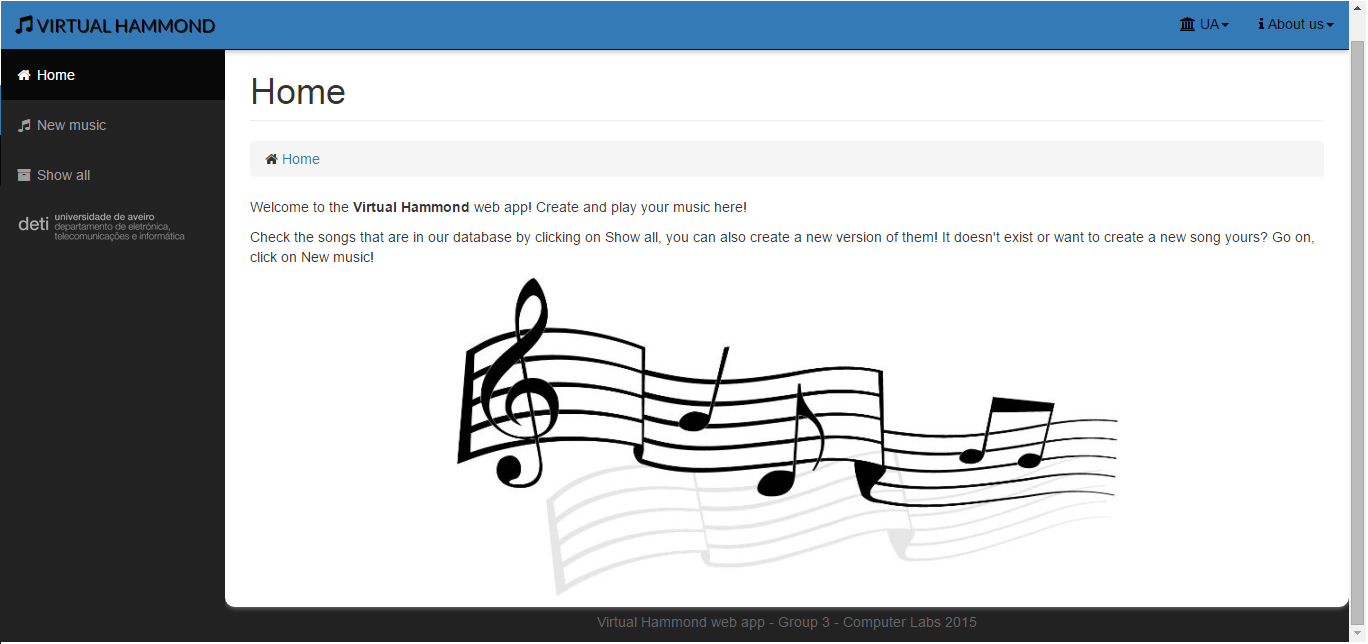
\includegraphics[scale=.3]{index.png}
 \caption{Página \textit{Home} da aplicação para \textit{desktop}.}
 \label{index}
\end{figure}

Na página \textit{New music} é possível ao utilizador criar uma nova música. O utilizador pode introduzir o nome da música, a pauta e o registo desejado. Desde que a pauta esteja no formato correto \acs{rtttl} e o registo satisfaça as condições exigidas, a música será criada com sucesso. Caso isso não aconteça, irá ser apresentada uma mensagem de erro. A escolha e aplicação de efeitos é uma decisão do utilizador. Isto irá criar automaticamente uma nova música com uma versão, que será guardada na base de dados, através do servidor.

Na página \textit{Show all} é feita uma listagem de todas as músicas existentes na base de dados. Para cada música, estão disponíveis três botões. O da direita, \textit{Get notes}, que serve para mostrar na mesma página a pauta dessa música. O botão central, \textit{New version}, levará o utilizador a uma página com um campo para escolher um registo e com os efeitos disponíveis. Depois de inseridos estes dados, será criada uma nova versão da música. Finalmente, o botão \textit{Show versions} listará todas as versões disponíveis daquela música, com indicação do registo e dos seus efeitos. Na página referida, o utilizador poderá carregar no botão \textit{Show info}, irá disponibilizar informação sobre a versão escolhida. Irá disponibilizar um gráfico com as notas da música (\autoref{showinfo}), um botão para ser criado e disponibilizado um ficheiro para audição, destacando-se a seguir o registo, os efeitos aplicados e os votos efetuados até ao momento, sendo possível efetuar votos (positiva ou negativamente) da versão em questão.

\begin{figure}
 \center
 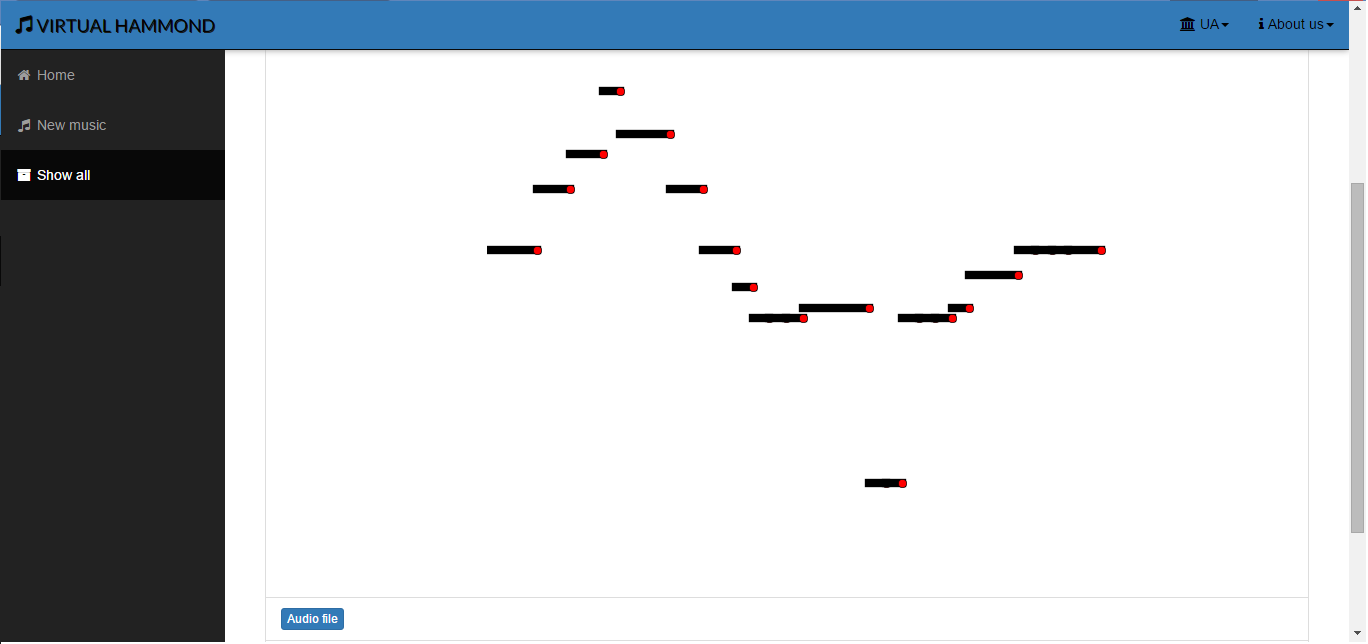
\includegraphics[scale=.3]{showinfo.png}
 \caption{Página \textit{Show Info} da aplicação para \textit{desktop}. Podemos ver o gráfico criado pela música "The Simpsons", bem como o botão para ouvir a música.}
 \label{showinfo}
\end{figure}

A aplicação \textit{mobile} foi desenhada para ser o mais similar possível à versão \textit{desktop}. Para se adaptar melhor aos \textit{smartphones} atuais, optámos por colocar um menu inferior horizontal, com os mesmos botões que na versão \textit{desktop} (embora a redirecionar para links diferentes). A página \textit{New music} tem as mesma funcionalidades, sendo bastante similar também na sua aparência em relação à \textit{New music} da versão \textit{desktop}. Também a página \textit{Show all} (\autoref{mshowall}) não difere em quase nada da versão \textit{desktop}, assim como as suas sucessivas ramificações através de botões existentes. A principal diferença é na maneira como as páginas fazem as transições entre si.
Usando a funcionalidade \textit{push} disponibilizada pelo \textit{Ratchet}, as páginas não comutam entre si de maneira usual. Só pode haver troca de página se houver um evento \textit{touch} nos botões disponibilizados. Quando isso acontece, apenas o conteúdo é alterado entre as páginas. A sua interação em computadores é apenas possível quando são ativados os \textit{touch events} através das opções de cada \textit{browser}.

\begin{figure}
 \center
 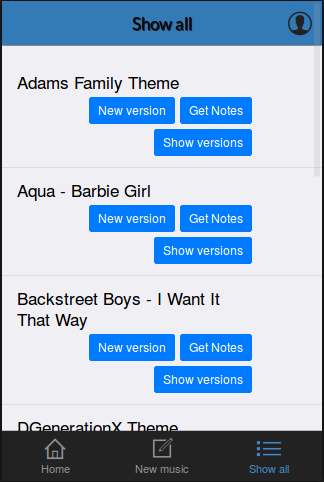
\includegraphics[scale=.5]{mshowall.png}
 \caption{Possível página \textit{Show all} da aplicação para \textit{mobile} (ecrã de tamanho 320x480).}
 \label{mshowall}
\end{figure}

\section{Aplicação Principal}
\paragraph{ } A aplicação principal é o módulo responsável por interligar o ambiente apresentado ao utilizador pela interface ao núcleo de processamento e armazenamento de informação, como a base de dados e os módulos de interpretação e sintetização. A sua estrutura pode ser subdividida em três partes: módulos importados, funções de serviços \textit{Cherrypy} e configuração do servidor.

Os módulos utilizados nesta aplicação são orientados para as necessidades e especificidades do código produzido e apresentam as seguintes funções:
\begin{itemize}
  \item \textit{sqlite3}: disponibiliza uma interface entre a aplicação desenvolvida em linguagem Python e a base de dados relacional do tipo \textit{SQLite};
  \item \textit{os} e \textit{os.path}: permite a manipulação de ficheiros e diretórios no ambiente Python;
  \item \textit{cherrypy}: permite o desenvolvimento de aplicações Web, apresentando uma interface de disponibilização de um servidor \ac{http};
  \item \textit{sys}: garante o acesso a variáveis de sistema e de do interpretador;
  \item \textit{json}: usado na manipulação de objetos do tipo \acs{json};
  \item \textit{matplotlib.pyplot} as plt: biblioteca de criação de gráfico 2D (pode não funcionar corretamente quando utilizada em sistemas \textit{Windows});
  \item \textit{socket}: módulo que disponibiliza o acesso ao sockets de comunicação usados para a comunicação entre aplicações;
  \item \textit{urllib2}: permite a manipulação e ligação a URLs e redirecionamento de informação.
\end{itemize}

Para além destas bibliotecas existentes para o desenvolvimento em \textit{Python} estão definidas outras que foram implementadas especificamente para o projeto em questão:

\begin{itemize}
  \item \textit{from inter import interp}: usa a função \textit{interp} do módulo \textit{inter}, cuja função é a interpretação das pautas em formato RTTL:
  \item \textit{from graph\_creator import createForm}: usa a função \textit{createForm} do módulo \textit{graph\_creator} , responsável pela criação do gráfico de frequências das notas;
  \item \textit{from sint import sintetizador}: usa a função \textit{sintetizador} do módulo \textit{sint}, que permite formar a onda de cada música.
\end{itemize}

A configuração do servidor \textit{Cherrypy} assenta na definição dos diferentes recursos que podem ser invocados pela aplicação. São configurados aspetos como a localização de ficheiros, endereços de acesso  e definição da estrutura de caminhos da aplicação.

O acesso à aplicação está configurado de forma a que possa ser efetuado por qualquer dispositivo compatível através da rede. Num processo transparente para o utilizador e independente da sua localização a função \textit{get\_ip\_address} estabelece uma ligação ao domínio \textit{google.com}, que tem como único fim a possibilidade de obter o endereço IP da máquina que nesse momento disponibiliza a aplicação.
\lstinputlisting[language=Python, firstline=308, lastline=313]{../main_app.py}

Assim, o acesso pode ser feito através da rede, permitindo que os dispositivos, sejam eles fixos ou móveis possam interagir com a aplicação. No momento em que a aplicação é ativada, é apresentada a informação de acesso à aplicação, com a indicação dos passos a seguir para utilização por parte de dispositivos móveis. 
\begin{figure}
 \center
 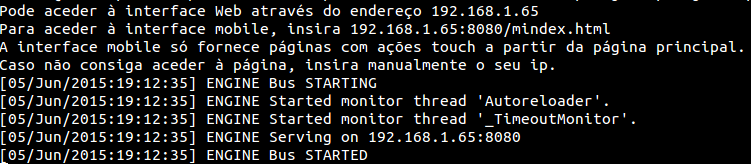
\includegraphics[scale=.5]{mensageminiciao.png}
 \caption{Mensagem apresentada aquando da iniciação da aplicação}
 \label{mensageminiciao}
\end{figure}

Os recursos que a aplicação usa e disponibiliza são muito importantes e necessitam de uma indicação clara em relação ao caminho para chegar até eles. O primeiro passo é o estabelecimento de uma estrutura baseada na localização absoluto da aplicação na máquina que a corre. Todos os recursos são chamados e disponibilizados com base nesta localização e num caminho relativo definido a partir daí. 
\lstinputlisting[language=Python, firstline=330, lastline=330]{../main_app.py}
A informação guardada pela variável \textit{current\_dir} permite a disponibilização de recursos como ficheiros \acs{css} ou \textit{JavaScript}, imagens, páginas \ac{html} e outros recursos através de um mapeamento estático do seu caminho. Como é possível verificar o caminho para o recurso é mapeado a partir da raiz definida através da variável \textit{current\_dir} e seguindo a orientação da estrutura indicada para cada caso.
\lstinputlisting[language=Python, firstline=331, lastline=335]{../main_app.py}
Em termos estruturais, a parte do processamento assenta em várias funções que disponibilizam serviços utilizados pela interface Web. A classe \textit{Root} engloba as funções \textit{index}, \textit{createSong}, \textit{createInterpretation}, \textit{listSongs}, \textit{listSongFiles}, \textit{getNotes}, \textit{updateVotes}, \textit{getWaveFile} e \textit{getWaveForm}.

As funções \textit{createSong} e \textit{createInterpretation}, são responsáveis pela criação de novas músicas ou de interpretações. Em termos de processamento apenas definem novas entradas na base de dados. A função \textit{listSongs} tem como finalidade a apresentação de dados sobre as diferentes músicas. As restantes funções são mais especificas, uma vez que utilizam parâmetros que identificam certos elementos. A função \textit{getNotes} disponibiliza a pauta de uma música, enquanto que a \textit{listSongFiles} permite acesso a vários dados de interpretações especificas, tal como efeitos e registos definidos, nome e número de votos. As funções \textit{getWaveFile} e \textit{getWaveForm} são responsáveis pelo processamento da criação dos ficheiros de som e imagem da interpretação. Como cada versão permite a atribuição de votos negativos e positivos a comunicação do número de votos em cada atualização é feita pela função \textit{updateVotes} que guarda a informação dos votos na base de dados.


\section{Interpretador de Pautas}
\paragraph{ } O interpretador de pautas (ficheiro "inter.py") irá receber uma \textit{String} (que representará a pauta) no formato \acs{rtttl}. Se não estiver no formato correto (se tiver espaços, se existirem mais ou menos do que dois ":", se houver um oitava sem nota, se houver uma nota ou uma oitava inexistentes, ...) lançará erro e retornará uma lista vazia. Foi feito um teste (usando \textit{pytest}) ao módulo, para garantir que assegurava o controlo dos erros, e que lançava as pautas corretas.

Caso esteja no formato correto, deverá armazenar as oitavas de referência, o pulso de referência e o andamento. Para cada nota, deverá fazer as contas à sua duração e à sua frequência (de acordo com uma \textit{Lookup Table} com todas as frequências possíveis de notas) e adicionar a uma lista estes pares. Cada nota deverá ter obrigatoriamente o seu tom. Poderá ter opcionalmente, antes da nota, o seu valor (se não tiver, presumir-se-há valor igual ao pulso de referência), ou depois da nota, um ponto (indica duração aumentada em 50\%) ou uma oitava (de 0 a 8, se não existir presume-se igual à oitava de referência). No final da pauta, essa lista será retornada.

\section{Sintetizador}
\paragraph{ } O sintetizador é responsável por formar a onda de cada música dado um conjunto de frequências e um certo registo. Recebendo uma lista de pares (duração, frequência) enviada pelo interpretador e um registo com nove algarismos, de 0 a 8 (verificado pelo \textit{JavaScript} existente), o sintetizador irá somar nove ondas com um certo múltiplo da frequência (1/2, 3/2, 1, 2, 3, 4, 5, 6, 8), ponderado pelo algarismo do registo nesse dígito, multiplicado pela amplitude e pela onda formada. Assim, é possível formar uma onda "analógica" com uma certa frequência de amostragem (44100 Hz) através de valores discretos.

A fórmula para este cálculo é

\begin{equation}
 \displaystyle\sum_{j=1}^{9} amplitude * \frac{reg[j]}{8} * \sin(\frac{2*\Pi*f*mul[j]*i}{rate})
 \label{F1} 
\end{equation} 

onde \textit{reg} é uma lista com os nove dígitos presentes no registo, \textit{f} é a frequência, \textit{mul} é uma lista com os múltiplos da frequência (descritos acima), i é um valor crescente que irá indicar o tempo e \textit{rate} será a frequência de amostragem, neste caso, 44100 Hz.


Após fazer a soma das ondas, a onda final terá que ser normalizada para depois poder ser enviada para o processador de efeitos para ser construído um ficheiro de formato \ac{wave}, que o sintetizador irá retornar o seu diretório ao servidor.

\section{Processador de Efeitos}
\paragraph{ } O processador (ficheiro "effects\_processor.py") deverá receber uma lista de tons pares (frequência, \textit{samples}) vindos do sintetizador, onde \textit{samples} são as amostras que possui a onda criada para essa frequência. O sintetizador irá criar um ficheiro no formato \textit{".wav"} e irá aplicar os seguintes efeitos, caso sejam pedidos pelo sintetizador:
\begin{itemize}
\item \textbf{Chorus}: Consiste em introduzir à atual onda outra onda de frequência ligeiramente superior (neste caso, 30 Hz), para cada frequência.
\item \textbf{Percussion}: Soma uma onda à atual com um múltiplo da frequência (neste caso, 4 vezes a frequência atual), com uma amplitude que decai ao longo do tempo, até se anular no instante final.
\item \textbf{Tremolo}: Faz variar ligeiramente a amplitude do sinal. Ao sinal atual, soma-o com ele próprio multiplicado com uma onda de amplitude mínima (neste caso, 0.3).
\item \textbf{Distortion}: Eleva cada tom da nota a um número natural. Por ser bastante inconfortável, o aplicado no processador de efeitos foi um efeito semelhante, mas mais eficaz (efeito original encontra-se comentado no código, cujos comentários podem ser retirados para testes). O efeito aplicado foi multiplicar o tom atual por ele próprio, multiplicado depois por uma amplitude mínima (0.01).
\item \textbf{Echo}: Aplica eco a uma música, somando um sinal futuro ao sinal atual, com uma atenuação na amplitude (no código tem amplitude 0.2).
\item \textbf{Envelope}: Deverá modelar cada nota de acordo com as características do instrumento, simulando assim mais fielmente a sua reprodução. Para frequências iguais seguidas, o efeito deverá ser anulado e a amplitude das notas deverá ser igual.
\end{itemize}


Para cada efeito, depois de aplicado, serão aplicados um de dois efeitos: o \textit{normalize}, que normalize as ondas com a amplitude máxima e mínima e evita \textit{clipping}, ou o efeito \textit{clipping}, que não o evita.

%%%%%%%%%%%%%%%%%%%%%%%%%%%%%%%%%%%%%%%%%%%%%%%%%%%%%%%
\chapter{Implementação}

\section{Interface Web}
\paragraph{ } A interface \textit{Web}, tal como mencionado no capítulo que apresenta a estrutura, foi implementada para uma versão \textit{desktop} e \textit{mobile}. Os ficheiros \textit{\*.html} das mesmas podem ser facilmente identificados nas pastas \textit{virtualhammond} no diretório principal. A versão \textit{desktop} é composta por sete ficheiros do tipo \acs{html}, nomeadamente: \textit{developers.html, index.html, newmusic.html, newversion.html, showall.html, showinfo.html e showversions.html}. Cada um destes ficheiros representa uma página com um propósito específico de interação com o utilizador. Os ficheiros respetivos à implementação \textit{mobile} começam pela letra \textit{m} seguidos pelo nome igual ao do ficheiro análogo para a implementação \textit{desktop}, à excepção do \textit{developers} que se apresenta sob um \textit{modal} disponível em cada página \textit{mobile}.

\subsubsection{Análise do código base constituinte}
\paragraph{ } Vejamos a implementação da página \textit{index.html} e serão comentadas as seguintes páginas apenas nas suas variações.\\

O \textit{head} da página \textit{index.html} é igual ao das restantes páginas. Aqui se apresenta o seu código: 
\lstinputlisting[language=HTML, firstline=14, lastline=38]{../virtualhammond/index.html}
Tal como se pode observar, as primeiras linhas destinam-se a definir os dados, \textit{meta}, que poderão ser usados como por exemplo por motores de busca. Define-se também o título e seguidamente os \textit{links} para os ficheiros \acs{css} e para a fonte da letra do título da página. Tal como mencionado no capítulo anterior foi usado um \textit{template Bootstrap} (nomeadamente, \textit{SB Admin} \url{http://startbootstrap.com/template-overviews/sb-admin/}).

Como forma de definir o \textit{layout} da página todo o conteúdo da mesma é editado dentro da \textit{div} com o \textit{id="wrapper"}. Dentro deste bloco a página é definida em dois blocos ao mesmo nível. O bloco de navegação:
\lstinputlisting[language=HTML, firstline=52, lastline=52]{../virtualhammond/index.html}
E o bloco com o conteúdo da página \textit{index.html}:
\lstinputlisting[language=HTML, firstline=106, lastline=106]{../virtualhammond/index.html}
É de notar que o que muda em todas as páginas \acs{html} (que pertencem à aplicação \textit{desktop}) é precisamente o conteúdo deste último bloco a ser mencionado, isto visto o esquema de navegação ser igual em todas.

A página \textit{mindex.html}, que se apresenta como página inicial da aplicação \textit{mobile}, contém um \textit{head} bastante semelhante ao referido anteriormente, diferindo em pequenos pormenores como os ficheiros \acs{css} e ficheiros que contém os \textit{Scripts} (ou seja, código \textit{JavaScript}). Em relação à aplicação \textit{desktop}, os \textit{Scripts} encontram-se no fim de cada página.

Na página \textit{New music} o conteúdo é apresentado num formato de introdução de dados que compõem uma música e um botão que confirma este formulário preenchido devidamente pelo utilizador. Baseia-se no seguinte código:
\lstinputlisting[language=HTML, firstline=127, lastline=146]{../virtualhammond/newmusic.html}
Este código encontra-se escrito da mesma forma na aplicação \textit{mobile}, à excepção das classes atribuídas. No entanto, em termos de aparência para o utilizador é praticamente igual.
Em ambos os casos, é utilizado \textit{JavaScript} para verificar se os dados preenchidos se encontram num formato correto, transferindo posteriormente cada campo para o servidor, o qual se encarrega de assegurar que é guardado na base de dados da aplicação. Na página \textit{newversion.html} o conteúdo é praticamente o mesmo, à excepção dos id's e das entradas que pedem o nome e a pauta da música (linhas 4 e 6 do código anterior), visto que já não são necessárias aquando da criação de uma nova versão.

Nas páginas \textit{showall.html} e \textit{showversions.html} o seu conteúdo encontra-se a cargo do \textit{JavaScript}, sendo que este recebe as músicas ou versões (dependendo do caso) e trata de as listar ordenadamente com as opções já referidas no capítulo referente à estrutura da interface \textit{Web}. O mesmo acontece com as páginas correspondentes na aplicação \textit{mobile}.

A página \textit{showinfo.html} apresenta o seu conteúdo com suporte no código \textit{JavaScript}, tendo como objetivo disponibilizar as informações relativas a uma versão específica. Irá ser listada a seguinte informação: o nome da música e versão, um gráfico das notas da música, um botão que permite gerar e reproduzir o seu ficheiro áudio através de um \textit{player}, o registo, os efeitos aplicados, o número de votos positivos e negativos atribuídos e a possibilidade de votar essa mesma versão através das imagens de \textit{like} e \textit{dislike}. A página correspondente na aplicação \textit{mobile} efetua as mesmas ações, diferindo apenas no pormenor do \textit{loading} implementado, que se apresenta mais simples e igualmente eficaz para o que se pretende.

Por último, a página \textit{developers.html} disponibiliza ao utilizador informações como os desenvolvedores da aplicação, a possibilidade de contactar cada um por e-mail e um pequeno texto informativo. Na aplicação \textit{mobile}, não existe uma página \acs{html} que faça correspondência direta com esta, sendo apresentada através de um \textit{modal} disponível em qualquer página \acs{html} desta versão mais reduzida e simplista, contendo apenas informações básicas sobre os criadores e uma referência ao repositório onde se encontra o desenvolvimento deste projeto.

Este módulo teve como principal contribuidor Luís Leira, que desenvolveu aproximadamente 62,5\% do módulo e contou com o apoio do Daniel Alves, desenvolvendo cerca de 32,5\%, sendo a restante percentagem dividida igualmente pelo Abel Neto e pelo Diogo Ferreira.

\section{Aplicação Principal}
\paragraph{ } A aplicação principal apresenta-se como um ponto de conexão entre os diferentes serviços. Sempre que o utilizador interage com o interface, despoleta uma funcionalidade da aplicação. Todo o código implementado neste módulo assenta na linguagem \textit{Python}, sendo evocadas várias bibliotecas para a execução das tarefas previstas. As funções desenvolvidas para responder aos pedidos da interface Web estão definidas dentro da classe \textit{Root}, que foi fixada na configuração como a raiz da estrutura.

Este módulo teve como principal contribuidor Daniel Alves, que desenvolveu aproximadamente 70\% do módulo e contou com a ajuda de Diogo Ferreira e Luís Leira numa contribuição de partes iguais.

\subsection{A implementação da base de dados e a função \textit{index}}
\paragraph{ } Neste projeto o armazenamento de informação é essencial pelo que foi necessário definir uma estrutura capaz de lidar com pedidos de forma eficaz. A flexibilidade que a linguagem Python tem facilita a interligação com a linguagem \ac{sql}. Desta forma é possível obter um programa organizado, fluído e coerente. A base de dados desenvolvida para esta aplicação assenta no módulo \textit{sqlite3} e foi construída com a estrutura apresentada na figura. Existem duas tabelas chamadas  \textit{musics} e \textit{interpretations}. A tabela \textit{musics} guarda informação relativa às diferentes músicas que são inseridas na aplicação. Os três campos que constituem esta tabela são \textit{music\_id}, que está definido como \textit{INTEGER PRIMARY KEY AUTOINCREMENT}, \textit{name} e \textit{stave} definidas como \textit{TEXT}. A tabela \textit{interpretations} guarda a informação das diferentes versões criadas para uma música. As versões caracterizam-se por poderem ser criadas com base em vários atributos diferentes. Para uma dada interpretação é possível definir um registo e combinar até seis efeitos diferentes. A tabela apresenta como chave primária o atributo \textit{interp\_id}, que está definido como \textit{INTEGER PRIMARY KEY AUTOINCREMENT}. Existem ainda campos para \textit{register} (\textit{INTEGER}), \textit{effect\_echo} (\textit{TEXT}), \textit{effect\_tremolo} (\textit{TEXT}), \textit{effect\_perc} (\textit{TEXT}), \textit{effect\_chorus} (\textit{TEXT}), \textit{effect\_dist} (\textit{TEXT}) e \textit{effect\_textttenv} (\textit{TEXT}). A informação das votações é guardada nas colunas \textit{posvotes} e \textit{negvotes} na forma de \textit{INTEGER DEFAULT} 0. Desta forma de cada vez que uma nova interpretação é criada este campo é preenchido de forma automática com o valor 0. A conexão entre as duas tabelas é assegurada pela definição de uma chave estrangeira \textit{music\_id} na tabela interpretations (\autoref{tabelasDB}). Desta forma é possivel obter dados como o nome ou a pauta de uma música a partir do \textit{interp\_id}.
 
\begin{figure}[h!]
 \center
 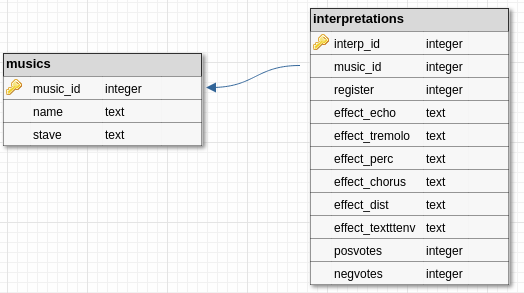
\includegraphics[scale=.5]{tabelasDB.png}
 \caption{Tabelas da base de dados}
 \label{tabelasDB}
\end{figure}

O comando \textit{CREATE TABLE IF NOT EXISTS} garante a criação da base de dados e respetivas tabelas apenas no caso de estas não existirem. 
\lstinputlisting[language=Python, firstline=26, lastline=36]{../main_app.py}
Algumas complicações com a codificação em \ac{utf8} obrigaram à introdução de um forçar de codificação, que assim garante um funcionamento adequado da aplicação.

No momento inicial de acesso à página o servidor corre o código descrito nesta função. Desta forma a página \textit{index.html} é disponibilizada pela função \textit{index} descrita na classe \textit{Root}. 

\subsection{As funções \textit{createSong} e \textit{createInterpretation}}
\paragraph{ }As funções \textit{createSong} e \textit{createInterpretations} têm como tarefa a criação de novas entradas nas tabelas da base de dados. Apesar do nome sugerir a criação do som da música ou da interpretação, estas funções fazem apenas leituras e atualizações. O acionamento da função \textit{createSong} dá-se sempre que o utilizador optar por criar uma nova música através da página \textit{newmusic.html} (ou \textit{mnewmusic.html} na versão mobile). Do lado da interface o utilizador introduz a informação do nome e pauta da música, que é guardada na tabela musics. Na aplicação criada foi considerado que a criação de uma música implica a criação da primeira versão. Assim é pedido ao utilizador um valor do registo e os efeitos a aplicar. Isto implica que a função \textit{createSong} tenha muitos parâmetros de entrada, no total nove.
\lstinputlisting[language=Python, firstline=47, lastline=50]{../main_app.py}
A interface Web garante a validade dos parâmetros introduzidos, à exceção da pauta. Esta é verificada pelo módulo interpretador de pauta. Caso o resultado da interpretação seja uma lista vazia a pauta não é aceite e a entrada para a música não é criada. 
\lstinputlisting[language=Python, firstline=57, lastline=73]{../main_app.py}
\begin{figure}[h!]
 \center
 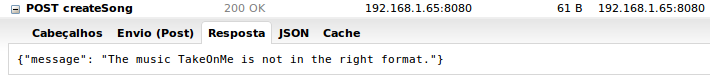
\includegraphics[scale=.55]{respostainsucesso.png}
 \caption{Aviso de pauta com formato errado}
 \label{respostainsucesso}
\end{figure}
A resposta nesta situação é uma mensagem que identifica a pauta como não estando no formato correto (\autoref{respostainsucesso}). Se a validação da pauta for positiva, o processo avança com a conexão à base de dados  e a inserção dos dados na tabela \textit{musics}. Para garantir a criação da primeira versão é necessário fazer o reencaminhamento para a função \textit{createInterpretation}. Isto é conseguido através do módulo \textit{urllib2}, que lida com o redirecionamento para outros links. Desta forma, os valores do registo e dos efeitos são passados à função \textit{createInterpretation}, que depois insere os dados de uma nova interpretação na tabela \textit{interpretations} da base de dados. 

Outro momento em que a função  \textit{createInterpretation} é chamada é aquando da criação de uma nova versão a partir de uma música existente na base de dados. Os valores que recebe são introduzidos na  tabela \textit{interpretations}, usando o comando \textit{INSERT INTO}. Cada parâmetro recebido é colocado na respetiva coluna, sendo que efeitos que não tenham sido escolhidos, recebem um valor de \textit{NONE}.

Um aspeto comum às funções implementadas é a forma como envia os dados para a interface Web. A comunicação é feita com base no formato \acs{json} e estrutura-se de forma a passar os elementos a apresentar (ou utilizar) na página, sendo os cabeçalhos de comunicação identificados com o respetivo formato. Um exemplo é o valor devolvido pela função \textit{createInterpretation}. Neste caso pretende-se dar uma informação de sucesso. O elemento \acs{json} é definido com a chave mensagem e  o respetivo valor.
\lstinputlisting[language=Python, firstline=106, lastline=106]{../main_app.py}


\subsection{As funções \textit{listSongs} e \textit{listSongFiles}}
\paragraph{ }O papel destas funções é de apresentar dados sobre músicas e interpretações existentes na base de dados. A apresentação de todas as músicas presentes na base de dados é conseguida com a função \textit{listSongs}. O facto de esta não necessitar de parâmetros define-a como uma função de apresentação de valores gerais sobre uma música. A consulta da base de dados é conseguida com recurso ao comando \textit{SELECT}, especificando os atributos a disponibilizar e como devem ser ordenados. A natureza mais complexa desta resposta obriga à criação de um elemento \acs{json} que incorpore todos os elementos encontrados. Neste caso, recorre-se a um elemento \acs{json} na forma de lista. Isto permite que cada linha da lista diga respeito a uma entrada da base de dados.

A função \textit{listSongFiles} tem uma incumbência mais especifica, uma vez que trata a informação referente a uma música. O parâmetro que recebe (\textit{musicid}) é usado na pesquisa dos dados e permite a obtenção dos valores relativos às diferentes interpretações existentes. A garantia de uma resposta não vazia é conseguida pela imposição de um elemento condicional. Caso este não se encontre vazio é devolvido no formato \acs{json}, recorrendo-se ao mesmo processo de codificação da \textit{string} concatenada com a informação pesquisada. 
\lstinputlisting[language=Python, firstline=154, lastline=162]{../main_app.py}
Na \autoref{JSONenviado} é possível ver parte da resposta enviada pela aplicação para interface Web na função \textit{listSongFiles}.
\begin{figure}[h!]
 \center
 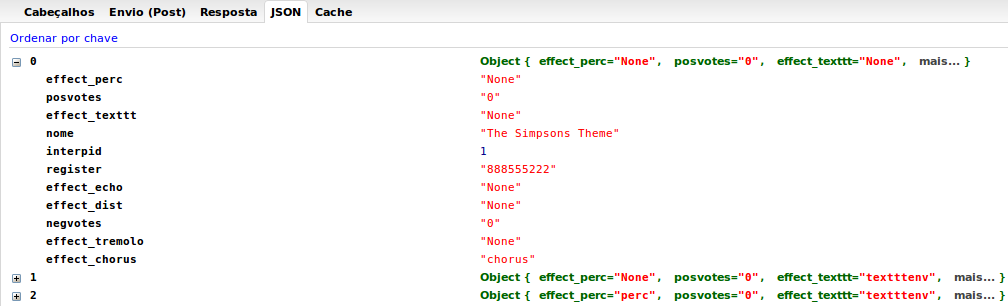
\includegraphics[scale=.38]{JSONenviado.png}
 \caption{Informação enviada para a Interface Web}
 \label{JSONenviado}
\end{figure}

\subsection{As funções \textit{getNotes} e \textit{updateVotes}}
\paragraph{ } A interação dos utilizadores com a aplicação vai para além da criação de músicas e respetivas interpretações. De forma a criar uma ligação maior às interpretações que criam, os utilizadores podem atribuir votos positivos ou negativos. A aplicação principal intervém neste processo apenas como módulo de armazenamento dos votos na base de dados. A função \textit{updateVotes} é acionada cada vez que os botões \textit{likes} ou \textit{dislikes} são premidos, recebendo a informação do respetivo número de votos. A escolha do botão implica a colocação da variável “contrária” a zero. Desta forma a função analisa os parâmetros \textit{neg} e \textit{pos} e decide qual necessita de ser atualizado. Na base de dados é possível definir um novo valor com o comando \textit{UPDATE} em conjunto com o comando \textit{SET}. 
\lstinputlisting[language=Python, firstline=207, lastline=211]{../main_app.py}
A função \textit{getNotes} tem como tarefa a pesquisa e envio da pauta relativa a uma música específica. O parâmetro \textit{musicid} que recebe permite a procura da respetiva pauta na tabela \textit{musics} da base de dados.

\subsection{As funções \textit{getWaveForm} e \textit{getWaveFile}}
\paragraph{ } Todas as funções mencionadas até ao momento têm como tarefa a pesquisa, inserção ou atualização da base de dados, não sendo produzidos ficheiros com os quais o utilizador pode interagir ou observar. As funções \textit{getWaveForm} e \textit{getWaveFile} são responsáveis por implementarem tarefas e chamarem módulos de criação de ficheiros de som e gráficos de notas.

A função \textit{getWaveForm} implementa a criação do gráfico definido por ramos das notas de uma música. Em termos de execução, a função usa o parâmetro recebido para pesquisar pela pauta na tabela \textit{musics} da base de dados. A pauta é interpretada pelo módulo interpretador de pauta e passado ao módulo de criação de gráficos. A função não devolve o ficheiro imagem, mas apenas o nome do ficheiro para a interface Web.
\lstinputlisting[language=Python, firstline=278, lastline=301]{../main_app.py}
A função \textit{getWaveFile} realiza a tarefa de gestão e passagem de valores aos vários elementos que estão envolvidos na criação do ficheiro de som. O processo começa pela pesquisa na base de dados da informação relativa à pauta, efeitos e registo de uma certa interpretação. A forma como os efeitos  se encontram armazenados na base de dados obriga a algum processamento antes de poder enviar os dados a outros módulos. A tabela \textit{interpretations} tem uma coluna para cada efeito, sendo este preenchido pelo nome do efeito, caso tenha sido selecionado, ou com \textit{NONE}, caso não tenha sido escolhido. Esta informação necessita de ser inserida numa lista, pelo que passa por um processo de validação e definição dos efeitos escolhidos.
\lstinputlisting[language=Python, firstline=243, lastline=256]{../main_app.py}
Tal como na função \textit{getWaveForm} a pauta é enviada ao interpretador de efeitos que devolve uma lista de tuplos. O processo de criação do ficheiro no formato \acs{wave} é despoletado pela chamada do módulo sintetizador, que recebe o valor do registo, a lista interpretada e a lista de efeitos. O resultado deste processo é um ficheiro de som, cujo caminho relativo é enviado para a interface Web.


\subsection{Criador de gráfico}
\paragraph{ } O módulo de criação do gráfico (ficheiro ”graph\_creator.py”) irá receber a lista produzida pelo  interpretador de pauta. Esta lista é constituída por pares (frequência, tempo), que no gráfico são representadas por linhas horizontais. Na manipulação e criação do gráfico é usado o módulo \textit{matplotlib}. Por forma a definir uma janela de visualização adequada para os dados de cada música procura-se os valores mínimos e máximos das frequências presentes na lista. O gráfico é constituído por linhas horizontais que unem dois pontos com duas coordenadas. Assim o ponto inicial corresponde ao par (\textit{xinitial}, \textit{freq}) e o ponto final ao par (\textit{xfinal}, \textit{freq}). Para o efeito vermelho na extremidade de cada ramo é sobreposto um segundo gráfico constituído apenas pelos pontos (\textit{xfinal}, \textit{freq}). Retirando os eixos e configurando a janela de visualização vertical com a ajuda dos valores mínimos e máximos das frequências é possível desenhar um gráfico como o da \autoref{graph}.
\begin{figure}[h!]
 \center
 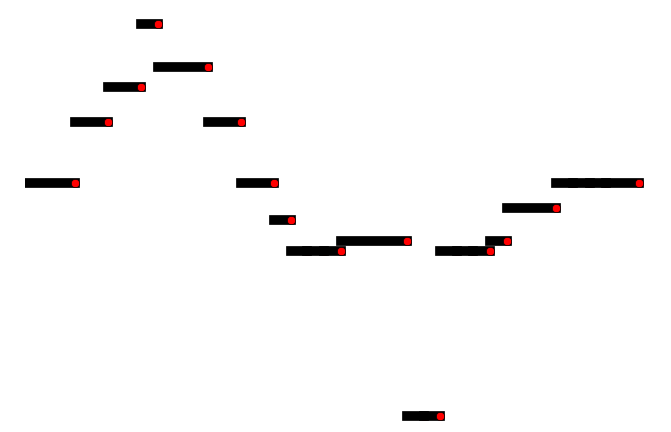
\includegraphics[scale=.38]{graph.png}
 \caption{Gráfico das frequências das notas}
 \label{graph}
\end{figure}
O gráfico é guardado localmente sendo possível visualizá-lo através da interface Web.
É importante referir que cada vez que o gráfico é criado e guardado é necessário limpar a variável \textit{plt}, para que se possa gerar um novo gráfico. A não existência desta condição leva à apresentação do mesmo gráfico para qualquer música.
\lstinputlisting[language=Python, firstline=30, lastline=55]{../graph_creator.py}

\section{Interpretador de Pautas}
\paragraph{ } O interpretador, após receber uma pauta em formato \textit{String}, começa por verificar se a pauta recebida tem dois ":". Se não tiver, lançará erro. Depois, tentará encontrar, após o primeiro ":", os valores de 'd', 'o' e 'b'. Caso haja algum erro no formato (espaço a mais, vírgula no local errado, valores inválidos), lançará erro. Caso não existam 'b', 'o' ou 'b', serão definidos os valores por defeito (d=4, o=5, b=63).

Após definido o formato inicial da pauta, tentará ler após o último ":". Assim, entrará numa iteração que, enquanto houver notas, fará o mesmo para todas. Primeiro, tenta ler o valor da nota. Caso o valor seja inválida, lançará uma erro. Caso esse valor não exista, será definido como valor o valor por defeito. Depois, tentará ler o tom da nota. Este elemento é o único que é obrigatório em cada nota, caso não exista, o programa lança erro. Quando deteta a nota, deteta também se é para aumentar meio-tom nessa nota, pelo sinal "\#" ou "\_".

Após ter a nota guardada, irá detetar a existência de ponto, que indicará se a duração dessa nota será aumentada em metade. Finalmente, irá detetar a oitava existente em cada nota. Caso seja inválida, lança um erro. Caso não exista, a oitava será a definida no início da pauta.

Para cada nota, será calculada uma duração ((4/(valor da nota)*(60/'b')). Se houver ponto, a duração será aumentada em metade. Também será calculada a frequência para cada nota, baseado numa \textit{Lookup Table}. Finalmente, os dois valores serão adicionados em forma (duração, frequência) a uma lista que será devolvida. Esse excerto de código está exposto abaixo:
\lstinputlisting[language=Python, firstline=155, lastline=178]{../inter.py}

Este módulo teve como principal contribuidor Diogo Ferreira, que desenvolveu o módulo a 100\%.


\section{Sintetizador}
O ficheiro \textit{sintetizador.py} vai definir uma função que tem como responsabilidade receber três registos, \textit{notes} que define as notas, \textit{register} que contém nove algarismos de zero a oito, \textit{effects} que define a lista de efeitos, todos eles definidos no \textit{main\_app.py}. Assim a função é definida como:
\lstinputlisting[language=Python, firstline=34, lastline=34]{../sint.py}

De seguida é verificado se os dados como \textit{reg} vêm no formato certo pelo seguinte código:
\lstinputlisting[language=Python, firstline=37, lastline=41]{../sint.py}

Com os dados disponíveis resta apenas implementar simplesmente a fórmula \ref{F1}. O código implementado não é mais do que o preenchimento de um array de \textit{samples}. 

Vejamos:
\lstinputlisting[language=Python, firstline=49, lastline=68]{../sint.py}

De notar também que na linha 18 do código acima podemos ver que cada \textit{sample} é enviada para a função \textit{normalize} que tem como objetivo limpar o possível \textit{clipping} da onda.
\lstinputlisting[language=Python, firstline=20, lastline=30]{../sint.py}

O valor máximo de amplitude suportado é 32767 devido ao número de bits disponíveis para cada \textit{sample}. Assim, a função \textit{normalize} procura pelo valor máximo da função e garante através da linha 10 do código acima que essa \textit{sample} assuma o valor 32767 e normaliza os restantes valores multiplicando-os pela constante de normalização que será o valor máximo permitido pelo sistema a dividir pela \textit{sample} de valor máximo.

Este módulo teve como principal contribuidor Abel Neto, que desenvolveu aproximadamente 80\% deste módulo, contando com a ajuda de Diogo Ferreira que obteve assim a restante percentagem.

\section{Processador de Efeitos}
\paragraph{ } O processador de efeitos começa por criar um ficheiro "song.wav" que será onde guardará a música criada. Será um diretório temporário, pois todas as músicas serão guardadas com o mesmo diretório, sobrepondo-se umas às outras, de modo a não sobrecarregar a aplicação devido ao tamanho ocupado por cada ficheiro no formato \acs{wave}.

Serão explicados detalhados todos efeitos, tal como são efetuados:
\begin{itemize}
\item \textbf{Chorus}: Adiciona uma onda com frequência ligeiramente superior à atual. \lstinputlisting[language=Python, firstline=88, lastline=89]{../effects_processor.py}
\item \textbf{Percussão}: Soma uma onda com o quádruplo da frequência, com a sua amplitude a decair ao longo do tempo. \lstinputlisting[language=Python, firstline=116, lastline=117]{../effects_processor.py}
\item \textbf{Tremolo}: Para variar a amplitude de sinal, este efeito soma a onda atual com uma onda de amplitude mínima multiplicada pelo valor atual da onda. \lstinputlisting[language=Python, firstline=66, lastline=67]{../effects_processor.py}
\item \textbf{Dist}: O efeito de distorção deveria elevar os valores da onda atual a um número natural. No entanto, como esse efeito ficaria pouco agradável, multiplicámos os valores da onda atual por ela própria, e depois por uma amplitude mínima. \lstinputlisting[language=Python, firstline=78, lastline=80]{../effects_processor.py}
\item \textbf{Echo}: Este efeito aplica eco a uma música, somando um sinal futuro ao sinal atual, com uma atenuação na amplitude. \lstinputlisting[language=Python, firstline=53, lastline=55]{../effects_processor.py}
\item \textbf{Envelope}: Este efeito modela nota a nota de acordo com o instrumento. Neste caso, a nota será crescente, de amplitude 0\% a 100\% no primeiro oitavo tempo da música. No segundo, a nota estabilizará em 50\% da sua amplitude. Continuará assim, até ao ultimo oitavo tempo da música, onde a amplitude descrescerá até 0. Caso a frequência da nota anterior seja igual à atual, o efeito anula-se nos dois primeiros oitavos tempos, mantendo-se sempre a 50\%. Caso a frequência da nota posterior seja igual à atual, o efeito anula-se nos último oitavos tempos, mantendo-se sempre a 50\%.
\lstinputlisting[language=Python, firstline=145, lastline=162]{../effects_processor.py}
\end{itemize}

Este módulo teve como principal contribuidor Diogo Ferreira, desenvolvendo este módulo a 100\%.

\part{Conclusão}
\chapter{Conclusão}
\paragraph{ } O resultado final deste projeto é evidenciado na interação utilizador-aplicação, aquilo que aos olhos do utilizador parece ser uma simples página \textit{Web} é o resultado de uma combinação bem estruturada de elementos que interagem entre si e providenciam ao utilizador uma experiência intuitiva. Neste ponto o objetivo do projeto é claramente cumprido. O ponto chave para esta conclusão está assente numa estrutura de código bem planeada o que permite o funcionamento adequado entre os vários elementos usados, nomeadamente as bases de dados, o servidor (\textit{ambiente Python}) e as páginas \textit{Web} (com os respetivos códigos \acs{html}, \acs{css} e \textit{Scripts}).

É de notar que com poucas ações o utilizador pode chegar às listas de músicas, pode criar uma nova, manipular resultados e ouvir o resultado final. Isto é fruto do cuidado em manter a aplicação intuitiva. É também importante referir o cuidado em manter esteticamente uma apresentação semelhante entre a aplicação \textit{desktop} e a aplicação \textit{mobile}. Também poderiam ser adicionadas posteriormente mais funcionalidades, como apagar uma música, adicionar imagens a músicas ou procurar por letras. Devido ao tempo limitado, não nos foi possível adicionar estas funcionalidade, que facilmen temte podem ser adicionadas posteriormente.

A rapidez na interação utilizador-aplicação \textit{web} é algo que deve ser alvo de comentário. Todos os painéis de navegação \textit{web} são rápidos na sua apresentação, porém o conteúdo variável de página para página já não reflete a rapidez anterior. Isto deve-se ao conteúdo ser invocado por um \textit{script} local que por sua vez invoca uma função do lado do servidor, que interage com a base de dados, que finalmente enviará o conteúdo em bruto para ser processado pelo \textit{script} para ser apresentado ao utilizador. Este processo é moroso principalmente na geração de uma música (em média 5 a 7 segundos).

Foi tido em conta o facto de, durante a escrita de todos os módulos, terem sido adicionados comentários para que o código escrito seja de fácil compreensão Sempre que alguma funcionalidade fosse implementada, era pedido \textit{feedback} a todos os elementos do grupo, para saber se a solução implementada era a mais correta e como podia ser melhorada. Houve grande interação por parte de todos os membros do grupo, principalmente quando algum tinha dificuldades em escrever alguma parte que lhe era designada. Foram algumas as vezes que o grupo se juntou, onde o desenvolvimento de cada módulo era contribuído por praticamente todos os elementos, algo que não é possível constatar através do sistema de controlo de versões, mas que é oportuno referir. Principalmente nas últimas semanas houve grande cooperação para a finalização da interface \textit{Web} e da aplicação principal. Assim, considera-se cumprido o projeto pedido ainda com alguma margem dentro das datas limite.


%%%%%%%%%%%%%%%%%%%%%%%%%%%%%%%%%
\chapter*{Acrónimos}
\begin{acronym}
\acro{rtttl}[\textit{RTTTL}]{Ring Tone Text Transfer Language}
\acro{json}[\textit{JSON}]{JavaScript Object Notation}
\acro{html}[\textit{HTML}]{HyperText Markup Language}
\acro{http}[\textit{HTTP}]{Hypertext Transfer Protocol}
\acro{css}[\textit{CSS}]{Cascading Style Sheets}
\acro{wave}[\textit{WAVE}]{WAVEform audio file format}
\acro{sql}[\textit{SQL}]{Structured Query Language}
\acro{utf8}[UTF-8]{8-bit Unicode Transformation Format}
\end{acronym}

\end{document}
